\documentclass{article}
\usepackage[utf8]{inputenc}
\usepackage[margin=1in]{geometry} % Ajusta los márgenes a 1 pulgada
\usepackage{graphicx}
\usepackage{listings}
\usepackage{xcolor}
\usepackage{hyperref}
\usepackage{tikz}
\usetikzlibrary{shapes.multipart}

\definecolor{codegreen}{rgb}{0,0.6,0}
\definecolor{codegray}{rgb}{0.5,0.5,0.5}
\definecolor{codepurple}{rgb}{0.58,0,0.82}
\definecolor{backcolour}{rgb}{0.95,0.95,0.92}

\lstdefinestyle{mystyle}{
    backgroundcolor=\color{backcolour},
    commentstyle=\color{codegreen},
    keywordstyle=\color{magenta},
    numberstyle=\tiny\color{codegray},
    stringstyle=\color{codepurple},
    basicstyle=\ttfamily\small,
    breakatwhitespace=false,
    breaklines=true,
    captionpos=b,
    keepspaces=true,
    numbers=left,
    numbersep=5pt,
    showspaces=false,
    showstringspaces=false,
    showtabs=false,
    tabsize=2
}

\lstset{style=mystyle}

\title{Convolutional Neural Networks – Lab 4}
\author{RUBEN MARTINEZ GONZALEZ}
\date{\today}

\begin{document}

    \maketitle


    \section{indicaciones}\label{sec:indicaciones}
    Implementar una Red Neuronal Artificial Multiclase para la clasificación de imágenes de dígitos
    del 0 al 9 escritos a mano (handwriting digit recognition).
    La base de datos (mnist.txt) contiene 5000 muestras de imágenes de dígitos escritos a mano

    Cada renglón de la base de datos consiste en 785 elementos separados por comas, donde los
    primeros 784 valores identifican los pixeles de la imágen del dígito, y el último valor del renglón
    indica la clase a la que pertenece esa muestra. Los renglones están separadas por un “enter”.
    El vector renglón de 784 valores representan una imagen de 28 x 28 pixeles. Los primeros 28
    valores del vector,representan la primera columna de pixeles de la imagen, los siguientes 28
    valores representan la segunda columna de pixeles, y así sucesivamente

    El objetivo principal es implementar una red neuronal (NN) artificial multiclase de
    retropropagación para clasificar las imágenes de dígitos del 0 al 9 escritos a mano. Las
    características de entrada de la NN son los 784 pixeles de la imagen. Para este trabajo sólo se
    utilizarán las primeras 1000 muestras de imágenes de la base de datos. Para entrenar a la NN
    (ajustar parámetros o pesos) utilizar las primeras 900 imágenes y las 100 restantes serán para
    probar el desempeño de la red. Calcular el error de la función de costo para cada época.
    Presentar en un reporte la descripción del problema, el método utilizado (incluyendo
    arquitectura de la NN, su función de costo, gradientes, etc.), resultados y comentarios.
    Asimismo, entregar el código fuente para ser compilado y evaluado.
    Como resultados, mostrar el porcentaje de reconocimiento final de la NN, esto es el porcentaje
    de aciertos de clasificación para las 100 nuevas muestras. Mencionar algunos de los errores de

    clasificación indicando la clase obtenida por la NN comparada con su verdadera clase. Graficar,
    con un graficador de su preferencia, los valores de costo obtenidos en cada época para observar
    el descenso del error durante el entrenamiento.
    Presentar en el reporte la porción del código correspondiente a la función de costo y la
    actualización de pesos.
    Al ejecutar el código fuente, debe cargar el modelo NN entrenado y realizar el proceso de
    prueba con las 100 nuevas muestras. Desplegar en pantalla: el porcentaje de reconocimiento
    de la red neuronal artificial en la prueba


    \section{introducción}\label{sec:introduccion}
    En este informe, se presenta el trabajo realizado en el laboratorio 4 de Redes Neuronales Convolucionales.

    \noindent
    La solución se implementó en Python utilizando la biblioteca NumPy para el procesamiento de matrices,
    Matplotlib para la visualización de gráficos y Scikit-learn solo para la separación de los datos en conjuntos de entrenamiento y prueba.
    La implementación está desplegada en un notebook de Google Colab, el cual se puede acceder a través del siguiente enlace:
    \texttt{%
        \href{https://drive.google.com/file/d/1G7FsF-o0YyQpEuUWFcWKjgZJbzFlSa0B/view?usp=sharing}{%
            Colab}%
    }


    \section{Procesamiento de datos}\label{sec:Procesamiento-de-datos}

    \subsection{Descripción}\label{subsec:descripcion}
    El procesamiento realizado para interpretar y segmentar los datos de la base de datos de mnist.txt se describe a continuación:
    \begin{itemize}
        \item Se lee el archivo mnist.txt y se invoca la función load\_data para cargar los datos en memoria.
        \item La función load\_data recibe como parámetro la ruta del archivo y retorna dos listas, una con las características de las imágenes y otra con las etiquetas de las imágenes.
        \item La función load\_data extrae las características de todos los primeros 784 valores de cada renglón y las etiquetas del último valor de cada renglón.
        \item Para visualizar una imagen aleatoria de los datos extraídos de mnist.txt se genera un índice aleatorio
        y se invoca la función visualize\_image pasando como parámetros las características (784 pixeles) y la etiqueta de la imagen correspondiente al índice aleatorio.
        \item Luego se visualiza la imagen en una matriz de 28x28 pixeles y se muestra la etiqueta correspondiente.
        \item Finalmente, se separan los datos en dos conjuntos, uno de entrenamiento y otro de prueba, utilizando la función train\_test\_split de la biblioteca scikit-learn.
        \item La separación de datos se realiza de un total de 1000 imágenes, 900 para entrenamiento (900\%) y 100 para prueba (10\%).
    \end{itemize}

    \subsection{Código implementado}\label{subsec:codigo-implementado}

    \begin{lstlisting}[language=Python, caption={carga de datos}, label={lst:load_data}]
def load_data(file_path):
    with open(file_path) as file:
        data = [line.strip().split(" ") for line in file]
        features = [np.asarray(data_point[:784], dtype=float) for data_point in data] # pixeles de la imágen
        labels = [float(data_point[-1]) for data_point in data]                       # clase a la que pertenece

    return features, labels

# Cargar los datos
file_path = "mnist.txt"
images, labels = load_data(file_path)
    \end{lstlisting}

    \begin{lstlisting}[language=Python, caption={Visualización de datos}, label={lst:visualize_data}]
def visualize_image(images, labels, n):
    if n >= len(images):
        print("El índice n está fuera del rango.")
        return
    image = images[n].reshape(28, 28)  # reconstruye la imagen en una matriz de 28x28
    label = int(labels[n])

    plt.imshow(image, cmap='gray')
    plt.title(f"Imagen del dígito: {label} índice:{n}")
    plt.axis('off')
    plt.show()

# Visualizar la imagen en la posición n
import random
n = random.randint(0, 5000)
visualize_image(images, labels, n)
    \end{lstlisting}
    \begin{lstlisting}[language=Python, caption={Separación de datos}, label={lst:split_data}]
X_train, X_test, Y_train, Y_test = train_test_split(np.asarray(images[:1000]), labels[:1000], test_size=0.1, shuffle=True)
    \end{lstlisting}
    \noindent

    \subsection{Resultados}\label{subsec:resultados}
    Al ejecutar el código se obtuvo la siguiente gráfica:
    \begin{figure}[h]
        \centering
        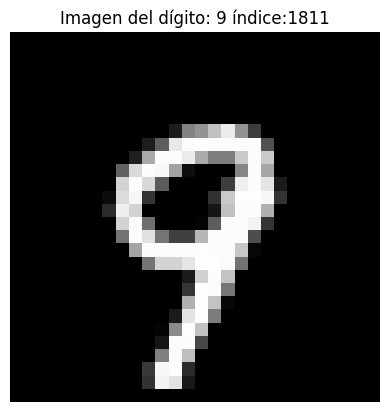
\includegraphics[width=0.5\textwidth]{img/ramdom_mnist}
        \caption{Gráfica de los datos de entrenamiento}
        \label{fig:plot_training_data}
    \end{figure}

    \clearpage


    \section{Descripción del problema}\label{sec:descripcion-del-problema}
    A partir de las imágenes (28 x 28) extraídas de la base de datos mnist.txt de dígitos del 0 al 9 escritos a mano y sus correspondientes etiquetas,
    se busca entrenar una red neuronal artificial para clasificar las imágenes en las 10 clases correspondientes a los dígitos del 0 al 9.
    El objetivo es implementar una red neuronal artificial multiclase de retropropagación para clasificar estas imágenes.


    \section{Método utilizado}\label{sec:metodo-utilizado}
    \begin{lstlisting}[language=Python, caption={Red Neuronal Artificial}, label={lst:neural_network}]
# Class to instatiate the model
class neural_network():
    def __init__(self, layers):
        self.layers = layers
        self.cost_function = CrossEntropy()

    def _forward_propagation(self, input_data):
        activation = Sigmoid()
        fwrd_result = [(None, input_data)]
        for l, layer in enumerate(self.layers):
            z = fwrd_result[-1][1] @ layer.weights + layer.bias
            a = activation(z)
            fwrd_result.append((z, a))
        return fwrd_result

    def _backward_propagation(self, labels, fwrd_pass):
        activation = Sigmoid()
        gradients = list()
        for layer_index, layer in reversed(list(enumerate(self.layers))): # Iteramos las capas de atrás hacia adelante
            current_weight = fwrd_pass[layer_index+1][1]
            if not gradients: #  capa de salida  derivada de la función de coste
                gradients.insert(0, self.cost_function.derivative(current_weight, labels) * activation.derivative(current_weight))
            else:
                previous_layer_weights = self.layers[layer_index + 1].weights.T
                gradients.insert(0, gradients[0] @ previous_layer_weights * activation.derivative(current_weight))
        return gradients

    def train(self, X, Y, learning_rate, epochs):
        history = list()
        print_interval = epochs // 5  # Imprimir la pérdida cada 20% del entrenamiento

        for epoch  in tqdm(range(epochs)):
            # calcular (a,z) para cada capa y almacenarlos en una lista
            forward_pass = self._forward_propagation(X/255)

            # Calcular la pérdida para seguir el rendimiento del modelo durante el entrenamiento
            loss = self.cost_function(forward_pass[-1][1], to_categorical(Y))

            # calcular las derivadas de la función de coste con respecto a los pesos y sesgos (gradientes)
            gradients = self._backward_propagation(to_categorical(Y), forward_pass)

            # Actualización de los pesos y sesgos
            for layer_index, _ in reversed(list(enumerate(self.layers))):
                layer = self.layers[layer_index]
                layer.bias -= learning_rate * np.mean(gradients[layer_index], axis=0, keepdims=True)
                layer.weights -= learning_rate * forward_pass[layer_index][1].T @ gradients[layer_index]

            history.append(loss)

            # Imprimir la pérdida cada 20% de las épocas
            if (epoch + 1) % print_interval == 0:
                print(f'Pérdida después de {((epoch+1)/epochs) * 100:.0f}% de las épocas: {loss}')

        return history

    def predict(self, X):
        # Realizamos la propagación hacia adelante
        forward_pass = self._forward_propagation(X)

        # Obtenemos las activaciones de la última capa
        last_layer_activations = forward_pass[-1][1]

        # Para cada conjunto de activaciones, seleccionamos el índice con la mayor activación
        predictions = [np.argmax(activations) for activations in last_layer_activations]

        return predictions
    \end{lstlisting}
    La solución propuesta para el problema de clasificación de imágenes de dígitos escritos a mano se implementó utilizando una red neuronal(NN) de retropropagación que se describe a continuación:
    \begin{itemize}
        \item La red neuronal implementada consta de 3 capas, una capa de entrada, una capa oculta y una capa de salida.
        \item La capa de entrada consta de 784 neuronas, una por cada pixel de la imagen.
        \item La capa oculta consta de 300 neuronas y la capa de salida consta de 10 neuronas, una por cada clase.
        \item La función de activación utilizada para las neuronas de la capa oculta es la función de activación sigmoide.
        \item La taza de aprendizaje utilizada es de 0.001 y el número de épocas es de 400.
        \item La función de costo utilizada es la función de costo de entropía cruzada.
        \item La actualización de los pesos se realiza utilizando el algoritmo de retropropagación.
        \item La red neuronal implementada consta de 3 métodos principales, el método \_forward\_propagation, el método \_backward\_propagation y el método train.
        \item El método \_forward\_propagation se encarga de realizar la propagación hacia adelante de las activaciones de las neuronas de la red.
        \item El método \_backward\_propagation se encarga de realizar la propagación hacia atrás de los gradientes de las neuronas de la red.
        \item El método train se encarga de entrenar la red neuronal utilizando los datos de entrenamiento y retorna el historial de la pérdida en cada época.
        \item El método predict se encarga de realizar la predicción de las clases de las imágenes de prueba.
    \end{itemize}

    \subsection{grafica de la estructura de la red neuronal}
    \begin{figure}[h]
        \centering
        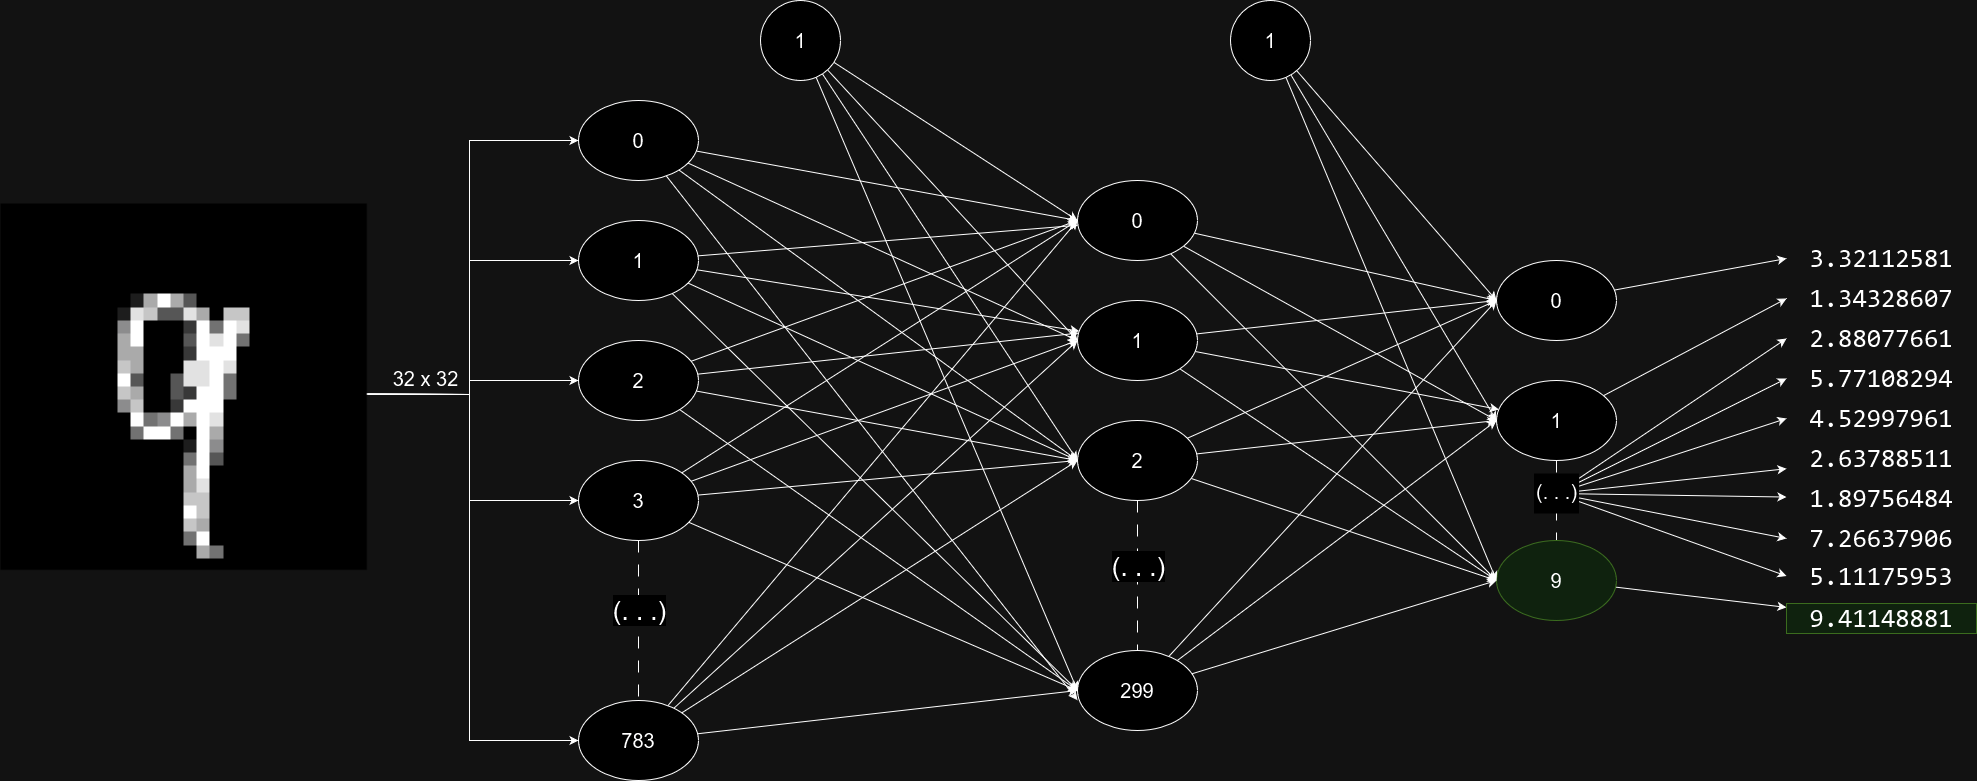
\includegraphics[width=0.99\textwidth]{img/red}
        \caption{Gráfica de la estructura de la red neuronal}
        \label{fig:red_neuronal}
    \end{figure}







    \section{Conclusiones}
    \noindent
    En este informe se presentó el trabajo realizado en el laboratorio 5 de Redes Neuronales Convolucionales.

\end{document}
